\chapter{Measurement of single top quark polarization in \textsl{t}~channel at 8~TeV}

\intro{A first measurement of the top quark spin asymmetry in t~channel, sensitive to the top quark polarization, is presented in this chapter. Proton-proton collision data at $\mathit{\sqrt{s}=8}$~TeV have been analyzed corresponding to about $\mathit{20~fb^{-1}}$. Events with an isolated muon are selected together with two or three jets for the final measurement. Events containing an isolated electron and jets have been studied as well. The normalized differential cross section is measured as a function of the polarization angle. From its shape, a spin asymmetry of $\mathit{0.26\pm0.03~(stat)\pm0.10~(syst)}$ is obtained. This is found to be compatible within $\mathit{2.0}$ standard deviations with the expected \gls{sm} spin asymmetry of $\mathit{0.44}$. The result has been published in Ref.~\cite{Khachatryan:2015dzz}. In a further step, the derivation of limits on anomalous couplings is illustrated by combining the result of this measurement with related ones.}


An overview of the strategy to measure the top quark spin asymmetry and derive limits on anomalous couplings is given in the following. After selecting events with an isolated muon or electron and two or three jets, two \glspl{bdt} are employed. The first one, \bdtqcd, is trained to reject events with fake leptons stemming from multijet production. The shape of multijet production is modeled by a template obtained from data in a sideband region for which the lepton isolation is inverted. Then, a two-component \gls{ml} fit to the \bdtqcd discriminant is performed to estimate the amount of multijet contamination after the event selection. The second \gls{bdt}, \bdttch, is optimized to separate signal from \wjets and \ttbar events. The amount of signal and background contributions is estimated through a second \gls{ml} fit to its discriminant. A signal-enriched phase space is obtained by applying an optimized selection on each of the \gls{bdt} discriminants resulting in a \gls{sb} ratio of about 90\%. The shape of the polarization angle, $\cos\theta^\star_{\mu}$, in data is unfolded to parton level after subtracting the remaining background contributions. This is repeated for each considered source of systematic uncertainty to estimate their impact on the measurement. The final measurement is performed in the muon channel only since in the electron channel, shortcomings in the modeling of the data-driven multijet template and an overall larger impact of systematic uncertainties are observed rendering its standalone result much less significant. The following description of the analysis is therefore primarily focused on the muon channel. 

The spin asymmetry is obtained from the differential cross section through a linear fit. The \TOPFIT program is utilized in a further step to set limits on anomalous Wtb couplings by combining the measured spin asymmetry with an inclusive cross section measurement in $t$~channel and a measurement of the W~boson helicity fractions in \ttbar production.



%##############################################
\section{Event selection and simulated samples}
%##############################################
\label{sec:polarization-selection}

Proton-proton collision data at $\sqrt{s}=8~\TeV$ are analyzed corresponding to $19.7~\invfb$ recorded with the \gls{cms} experiment in 2012. Events are triggered on the presence of a single muon or electron candidate. The employed single muon trigger requires an isolated muon candidate with $\pt>24~\GeV$ within the pseudorapidity range of $|\eta|<2.1$. The single electron trigger fires when an electron candidate with $\pt>27~\GeV$ within $|\eta|<2.5$ is detected that has to fulfill some additional quality criteria which correspond to an efficiency of 80\% for prompt electrons. Events are categorized into ``channels'' depending whether they have been triggered with the muon or electron trigger. For analysis, events in the muon channel have to contain one muon candidate with $\pt>26~\GeV$ within $|\eta|<2.1$ that passes the tight identification requirements. In the electron channel, events considered for analysis have to contain one electron candidate with $\pt>30~\GeV$ within $|\eta|<2.5$ where however the \gls{ecal} barrel-endcap transition region is excluded. In addition, the electron candidate has to fulfill the tight \gls{mva}-based identification requirements. To suppress fake leptons from multijet production, the muon candidate is required to be isolated with a relative \gls{deltabeta}-based isolation of $\muiso<12\%$ whereas the electron candidate has to have a relative \gls{effarea}-based isolation of $\eiso<10\%$. Events containing additional muons~($\pt>10~\GeV$, $|\eta|<2.5$, $\muiso<20\%$) or electrons~($\pt>20~\GeV$, $|\eta|<2.5$, $\eiso<15\%$) which pass corresponding loose identification criteria are rejected to suppress contributions from \zjets and dileptonic \ttbar production. 

Jets are clustered from \gls{pf} candidates with the anti-\kt algorithm using a distance parameter of $R=0.5$ while applying the \gls{chs} technique to remove the contamination of pileup tracks. \gls{pf} candidates belonging to preselected muons or electrons with a loose isolation are not clustered into the jets to prevent double counting. In addition, jets which are within $\Delta R<0.3$ to the selected tight lepton are ignored in the analysis. The reconstructed jet energy in data and simulation and the energy resolution in simulation are calibrated through dedicated \gls{jec} and \gls{jer} scale factors. Events containing in addition to a tight lepton two or three jets with $\pt>40~\GeV$ within $|\eta|<4.5$ that pass loss identification criteria are considered for analysis. B-tagging of jets is performed with the \gls{mva}-based \gls{csv} algorithm. The tagging of jets is restricted to $|\eta|<2.4$ since the algorithm operates only within the acceptance of the inner tracking system. In simulation an efficiency of about 50\% for tagging true b~jets with a mistagging rate of 0.1\% for other jets is found at the employed tight working point of the algorithm. The b-tagging efficiency is reweighted in simulation through scale factors to match the one measured in data. More details about the analysis objects, identification, and corrections have been described in Ch.~\ref{ch:reconstruction}.

After the selection, events are categorized per lepton channel as visualized in Fig.~\ref{fig:polarization-categorization}. The regions are labeled as ``$N\,\mathrm{j}~M\,\mathrm{t}$'' where $N$ denotes the number of selected jets and $M$ the subset of jets which are also b-tagged. Control regions dominated by either \wjets~(2j0t) or \ttbar~(3j1t, 3j2t) production are defined besides the signal region~(2j1t) as indicated in Fig.~\ref{fig:polarization-categorization}. The analysis was developed by validating the background modeling and optimizing the strategy using data in the control regions only. During this process, distributions of data in the signal region have not been used which is commonly referred to as ``blinding''. After the strategy is fixed the final measurement was conducted by unblinding the signal region while refraining from any further optimizations. Thus, the blinding procedure prevents a result-driven tuning of the analysis strategy which may otherwise bias the result.

\myfigure{\label{fig:polarization-categorization}Categorization of events depending on number of selected jets, number of b-tags, and the signal \gls{bdt} discriminant. The shaded regions are utilized in a template-based \gls{ml} fit as described in Sec.~\ref{sec:polarization-fit} for estimating the signal and background yields.}{
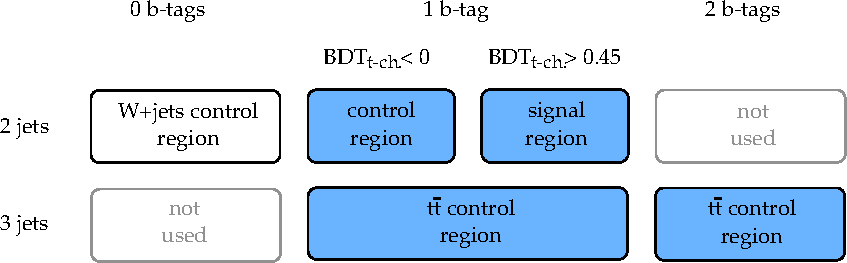
\includegraphics[scale=0.75]{figures/polarization/regions.pdf}
}

Various samples of simulated events for signal and background processes are generated. The default $t$-channel single-top-quark signal sample is generated in 5~\gls{fs} using the \POWHEG\,v1 generator interfaced with \PYTHIA\,6 for parton showering and \TAUOLA for tau decays. For comparisons, two additional, alternative signal samples are generated. One utilizes the \AMC generator interfaced with \PYTHIA\,8 in 4~\gls{fs} while the other employs the \COMPHEP generator interfaced with \PYTHIA\,6. A set of special samples with anomalous Wtb couplings is generated as well using the \COMPHEP generator for cross checking the analysis strategy. Samples containing single top quark events produced via tW and $s$~channel are generated with \POWHEG\,v1 interfaced with \PYTHIA\,6 and \TAUOLA. The major background processes, \wjets, \zjets, and \ttbar, are generated with the \MG generator interfaced with \PYTHIA\,6 and \TAUOLA as well. Samples with up to three~(\ttbar) or four~(\wjets,\zjets) additional partons at \gls{me} level are merged together using the \gls{mlm} procedure. For \wjets production, an alternative sample generated with the \SHERPA generator~\cite{Hoeche:2012ft} is employed for validation purposes. In this thesis, \wjets events are categorized based on their jet flavor content. Events with at least one heavy-quark flavored jet from either c, or b~quarks are abbreviated as ``\glsmark{whf}'' while events with only light-quark flavored jets~(g,u,d,s) are labeled as ``\glsmark{wlf}'' instead. Diboson production~(WW,WZ,ZZ) is a minor background and simulated with \PYTHIA\,6. The theoretical \gls{sm} cross sections used to normalize the samples are listed in Tab.~\ref{tab:polarization-theo-xsecs}. Throughout this chapter the individual signal and background templates are shown after they have been scaled to the result of a binned \gls{ml} fit to data~(Sec.~\ref{sec:polarization-fit}) and corrections to the simulated \wjets and \ttbar events~(Sec.~\ref{sec:polarization-modeling}) have been applied unless explicitly stated otherwise.


\mytable{\label{tab:polarization-theo-xsecs}Theoretical cross sections used to normalize the simulated samples.}{
\begin{tabular}{|l  r c l |}
\hline
process & $\sigma/\pb$ &\hspace{0.1cm} & accuracy \\
\hline
$t$~channel & $87.1~\pb$ & & approx. \gls{nnlo}~\cite{Kidonakis:2012db} \\
$s$~channel & $5.55~\pb$ && approx. \gls{nnlo}~\cite{Kidonakis:2012db}  \\
tW~channel & $22.2~\pb$ && approx. \gls{nnlo}~\cite{Kidonakis:2012db} \\
\ttbar & $252.9~\pb$ && \gls{nnlo} (using Top++\,2.0~\cite{Czakon:2011xx}) \\
$\mathrm{W}\to\ell\nu\mathrm{\,\mbox{+}\,jets}$ & $37\,509~\pb$ && \gls{nnlo} (using FEWZ~\cite{Gavin:2010az}) \\
$\mathrm{Z}/\gamma^{*}\to\ell^{\rmplus}\ell^{\rmminus}$, $m_{\ell\ell}>50~\GeV$ & $3\,504~\pb$ && \gls{nnlo} (using FEWZ~\cite{Gavin:2010az}) \\
WW & $54.8~\pb$ && \gls{nlo} (using MCFM\,5.8~\cite{Campbell:2010ff})\\
WZ & $33.2~\pb$ && \gls{nlo} (using MCFM\,5.8~\cite{Campbell:2010ff})\\
ZZ & $8.1~\pb$ && \gls{nlo} (using MCFM\,5.8~\cite{Campbell:2010ff})\\
\hline
\end{tabular}
}

Contributions from fake leptons produced in multijet events that survive the event selection are not simulated but estimated from data through the following procedure. The shape of multijet events per channel is extracted from a sideband region for which the isolation of the lepton is inverted in the event selection as $\muiso>20\%$ and $\eiso>15\%$, respectively. The resulting distribution of data after subtracting the remaining contamination by other processes serves as a template to model the shape of multijet production per observable. The amount of multijet production in signal and control regions is estimated by fitting the extracted template to data. The fit setup is described later in Sec.~\ref{sec:polarization-fit}. Figure~\ref{fig:polarization-qcd-template-antiiso} shows the distribution of the transverse W~boson mass in the 2j1t sideband region of the muon channel. The contribution of other processes in the sideband region amounts to a contamination of only 9\% (2\%) in muon (electron) channel respectively. The resulting multijet template after it has been fitted to data in the 2j1t region of the muon channel is shown in Fig.~\ref{fig:polarization-qcd-template-iso}. The data-driven procedure yields a good description of the unknown multijet shape in the signal region here.

\myfigure{\label{fig:polarization-qcd-template}Distributions of the transverse W~boson mass in muon channel: (a)~antiisolated sideband region for extracting the multijet template; (b)~resulting distribution in the 2j1t region after scaling the extracted template to data through a \gls{ml} fit.}{
\subfloat[\label{fig:polarization-qcd-template-antiiso}]{\adjincludegraphics[height=4.8cm,trim={0 0 {0.16\width} 0},clip]{figures/polarization/beforeBgCorr/2j1t/muon_2j1t_mtw_qcdnone_antiiso_nol.pdf}}
\subfloat[\label{fig:polarization-qcd-template-iso}]{\adjincludegraphics[height=4.8cm,trim={0 0 {0.\width} 0},clip]{figures/polarization/afterBgCorr/2j1t/muon_2j1t_mtw_qcdnone.pdf}}
}

Distributions of the reconstructed top quark mass in muon and electron channel are presented in Fig.~\ref{fig:polarization-topmass} after the event selection and the estimation of multijet events have been performed. In control regions containing no or more than one b-tagged jet, the jet with the highest value of the \gls{csv} discriminant is associated to the top quark decay to calculate the top quark mass.  The presented distributions demonstrate that data is well described by the simulated event samples and the data-driven multijet templates in control and signal regions for electron and muon channel.

In a top quark mass range of about $150\range190~\GeV$ the distributions display a peak for single top quark production as expected. For \ttbar production, the selected b-tagged jet may not be always associated with the corresponding lepton from a top quark decay. Hence, its distributions results into a peak with a wider tail. Unfortunately, the event selection also leads to a similar peak-like shape for the \wjets background although with an even longer tail. From these distributions it can be concluded that a simple selection on the top quark mass is insufficient to select a signal-enriched phase space. Therefore, two \glspl{bdt} are trained for separating signal from background events more efficiently as detailed in the next section.

\myfigure[p]{\label{fig:polarization-topmass} Distributions of the reconstructed top quark mass in (left column)~electron and (right column)~muon channel. Top row: 2j0t \wjets control region; middle row: 2j1t region; bottom row: 3j1t \ttbar control region. The top quark \pt reweighting~(Sec.~\ref{sec:polarization-modeling}) is exceptionally not applied here.}{
\subfloat[]{\adjincludegraphics[height=4.8cm,trim={0 0 {0.16\width} 0},clip]{figures/polarization/beforeBgCorr/2j0t/electron_2j0t_top_mass_qcdnone_nol.pdf}}
\subfloat[]{\adjincludegraphics[height=4.8cm,trim={0 0 {0.\width} 0},clip]{figures/polarization/beforeBgCorr/2j0t/muon_2j0t_top_mass_qcdnone.pdf}}\\
\subfloat[]{\adjincludegraphics[height=4.8cm,trim={0 0 {0.16\width} 0},clip]{figures/polarization/beforeBgCorr/2j1t/electron_2j1t_top_mass_qcdnone_nol.pdf}}
\subfloat[]{\adjincludegraphics[height=4.8cm,trim={0 0 {0.\width} 0},clip]{figures/polarization/beforeBgCorr/2j1t/muon_2j1t_top_mass_qcdnone.pdf}}\\
\subfloat[]{\adjincludegraphics[height=4.8cm,trim={0 0 {0.16\width} 0},clip]{figures/polarization/beforeBgCorr/3j2t/electron_3j2t_top_mass_qcdnone_nol.pdf}}
\subfloat[]{\adjincludegraphics[height=4.8cm,trim={0 0 {0.\width} 0},clip]{figures/polarization/beforeBgCorr/3j2t/muon_3j2t_top_mass_qcdnone.pdf}}
}



%##############################################
\section{Training of Boosted Decision Trees}
%##############################################
\label{sec:polarization-bdt-training}

Two \glspl{bdt} are trained in this analysis whose output is utilized two-fold, i.e. for estimating the amount of signal and background events in data and to obtain a signal-enriched phase space. The first \gls{bdt}, labeled \bdtqcd, is trained to reject background events stemming from multijet production. Simulated $t$-channel single top quark events are set as signal whereas data events in the sideband region, from which the multijet template is extracted, are set as background in its training. The gradient boosting procedure is chosen with a relatively low shrinkage of 10\%. The number of single decision trees is restricted to 50 while each tree is kept shallow with a maximum depth of two. The minimum node size is set to 250 events and the number of scanned working points per node is restricted to 200. These settings are not optimized to yield the best discrimination power but instead are motivated to protect well against overtraining. Overtraining is a particular concern here since the usage of data events for training may not reflect the actual distribution of multijet events in the signal region in great detail. Multiple \gls{bdt} candidates are trained to assess which set of input observables yields the best rejection of multijet events with the final discriminant. In addition, input observables which are found to be correlated with the polarization angle or with other input observables are excluded from the training. This optimization resulted in the following list of input observables for training:

\begin{itemize}
\item the reconstructed invariant mass of the top quark candidate;
\item the transverse mass of the W~boson candidate before solving for the unknown neutrino $p_{z}$ component since this modifies \pvmiss in the case of complex solutions, \mtw;
\item the missing transverse energy, \met;
\item the transverse momentum of the untagged spectator jet~(\jprime);
\item the event isotropy which is defined as $(s_\mathrm{max}-s_\mathrm{min})/s_\mathrm{max}$ with $s=\sum_{i}^\scriptn{\ell,\,\mathrm{jets}}\big|\,\vec{n}\cdot\vec{p}_{i}\big|$ where the unit vector $\vec{n}=(\cos\phi,\sin\phi)$ is chosen in the transverse plane such that it either maximizes or minimizes $s$.
\end{itemize}

The \gls{bdt} is trained on events in the 2j1t region only whereas the resulting discriminator is evaluated in control regions as well. Distributions of \mtw, the spectator jet $\pt$, and the event isotropy are presented in Fig.~\ref{fig:polarization-qcdinputs}. Other input observables are shown in Figs.~\ref{fig:polarization-qcd-template} and~\ref{fig:polarization-topmass} above. Distributions of the resulting \gls{bdt} discriminants in electron and muon channel are shown Figs.~\ref{fig:polarization-bdt-qcd-ele} and~\ref{fig:polarization-bdt-qcd-mu} respectively. A fair agreement is observed between data and simulation for the considered input observables and the final discriminant.

\myfigure{\label{fig:polarization-qcdinputs}Distributions of some input observables of the \bdtqcd and \bdttch discriminants as indicated in 2j1t muon channel: (a)~missing transverse energy; (b)~transverse momentum of untagged spectator jet; (c)~event isotropy; (d)~transverse momentum of b~tagged jet.}{
\subfloat[\bdtqcd and \bdttch]{\adjincludegraphics[height=4.8cm,trim={0 0 {0.16\width} 0},clip]{figures/polarization/afterBgCorr/2j1t/muon_2j1t_met_qcdnone_nol.pdf}}
\subfloat[\bdtqcd and \bdttch]{\adjincludegraphics[height=4.8cm,trim={0 0 {0.\width} 0},clip]{figures/polarization/afterBgCorr/2j1t/muon_2j1t_ljet_pt_qcdnone.pdf}}\\
\subfloat[only \bdtqcd]{\adjincludegraphics[height=4.8cm,trim={0 0 {0.16\width} 0},clip]{figures/polarization/afterBgCorr/2j1t/muon_2j1t_isotropy_qcdnone_nol.pdf}}
\subfloat[only \bdttch]{\adjincludegraphics[height=4.8cm,trim={0 0 {0.\width} 0},clip]{figures/polarization/afterBgCorr/2j1t/muon_2j1t_bjet_pt_qcdnone.pdf}}
}

In a preliminary version of this analysis~\cite{CMS-PAS-TOP-13-001}, events with $\mtw>50~\GeV$ ($\met>45~\GeV$) are selected in muon (electron) channel respectively to reject multijet events. Here, the working points of the \bdtqcd discriminant have been chosen such that a similar signal selection efficiency is obtained per channel. A comparison of the working point performances is presented in Tab.~\ref{tab:polarization-qcdeff}. The new \bdtqcd discriminant allows to reject about twice as much multijet events with respect to \mtw, \met while retaining approximately the same amount of signal events.

\mytable{\label{tab:polarization-qcdeff}Selection efficiencies of multijet and signal events using \bdtqcd, \mtw, and \met working points where the latter two were used in a preliminary version of the analysis.}{
\begin{tabular}{|r | c c | c c |}
\hline
& \multicolumn{2}{c|}{Muon channel} & \multicolumn{2}{c|}{Electron channel}\\
Process    & $\mtw>50~\GeV$ & $\bdtqcd>-0.15$ & $\met>45~\GeV$ & $\bdtqcd>0.15$ \\
\hline
Multijet  & 15\% & 7.7\%  & 7.6\% & 4.4\% \\
Signal   & 70\% & 71\%   & 51\%  & 52\% \\
\hline
\end{tabular}
}

The second \gls{bdt}, \bdttch, is trained to separate signal events from \wjets and \ttbar production which are the major background processes after applying the multijet rejection selection. It is configured as follows. The gradient boosting method is employed with a shrinkage of 40\%. In total, 200~shallow single decision trees with a maximum depth of two are trained. The minimum node size is set to 100 events and the number of scanned working points per node is set to 50. To mitigate a potential lack in the training statistics of the background samples, additional simulated \wjets and \ttbar events from the 2j0t and 3j2t control regions are added to the training, respectively. In particular, this increases the statistics of simulated events with W+light flavored jets which is relatively low in the 2j1t region but may in fact be larger in data due to mistagging. The following ten observables have been chosen as input:

\begin{itemize}
\item the reconstructed invariant mass of the top quark candidate;
\item the missing transverse energy, \met;
\item the transverse mass of the W~boson candidate before solving for the unknown neutrino $p_{z}$ component, \mtw;
\item the transverse momentum of the lepton;
\item the transverse momentum of the b-tagged jet;
\item the invariant mass of the b-tagged jet from the summed momenta of the clustered \gls{pf} candidates;
\item the absolute pseudorapidity of the untagged spectator jet~(\jprime);
\item the absolute pseudorapidity of the b-tagged jet;
\item the invariant mass of the top quark and spectator jet system, $\sqrt{\hat{s}}=\big|\vec{p}_{\mathrm{top}}+\vec{p}_{\jprime}\big|$\,;
\item the transverse momentum of the hadronic final-state system~(\glsmark{hfs}), $\big(\vec{p}_{\jprime}+\vec{p}_{\mathrm{b}}\big)_\mathrm{T}$\,.
\end{itemize}

These observables have been chosen for the training because they exhibit only a low correlation with the polarization angle. A bias may otherwise occur since the \gls{bdt} is trained with a sample of simulated signal events in which a \gls{sm} coupling structure is assumed. In the worst case, the \gls{bdt} may select events in such a way that it artificially reproduces the shape of the expected polarization angle in data. Choosing uncorrelated observables makes the \gls{bdt} training blind to the actual distribution of the polarization angle instead. The distributions of some input observables are shown in Fig.~\ref{fig:polarization-tchinputs} after selecting events with $\bdtqcd>-0.15$ in 2j1t muon channel. The other input observables are presented in Figs.~\ref{fig:polarization-qcd-template}, \ref{fig:polarization-topmass}, and~\ref{fig:polarization-qcdinputs} above. The resulting discriminants are shown in Figs.~\ref{fig:polarization-bdt-tch-ele} and~\ref{fig:polarization-bdt-tch-mu} in the electron and muon channel respectively. Overall, a good description of data with simulation is observed. The \bdttch discriminant yields an \gls{auc} of 29\% for separating signal from \wjets and \ttbar events in both channels.


\myfigure[p]{\label{fig:polarization-tchinputs}Distributions of some input observables to the \bdttch discriminant in 2j1t muon channel: (a)~transverse momentum of the muon; (b)~invariant mass of the b-tagged jet; (c,d)~absolute value of the untagged and b-tagged jet pseudorapidities; (e)~invariant mass of the top quark and spectator jet system; (f)~\pt of the hadronic final state system.}{
\subfloat[]{\adjincludegraphics[height=4.8cm,trim={0 0 {0.16\width} 0},clip]{figures/polarization/afterBgCorr/2j1t/muon_2j1t_lepton_pt_qcdbdt_nol.pdf}}
\subfloat[]{\adjincludegraphics[height=4.8cm,trim={0 0 {0.\width} 0},clip]{figures/polarization/afterBgCorr/2j1t/muon_2j1t_bjet_mass_qcdbdt.pdf}}\\
\subfloat[]{\adjincludegraphics[height=4.8cm,trim={0 0 {0.16\width} 0},clip]{figures/polarization/afterBgCorr/2j1t/muon_2j1t_ljet_abseta_qcdbdt_nol.pdf}}
\subfloat[]{\adjincludegraphics[height=4.8cm]{figures/polarization/afterBgCorr/2j1t/muon_2j1t_bjet_abseta_qcdbdt.pdf}}\\
\subfloat[]{\adjincludegraphics[height=4.8cm,trim={0 0 {0.16\width} 0},clip]{figures/polarization/afterBgCorr/2j1t/muon_2j1t_shat_mass_qcdbdt_nol.pdf}}
\subfloat[]{\adjincludegraphics[height=4.8cm,trim={0 0 {0.\width} 0},clip]{figures/polarization/afterBgCorr/2j1t/muon_2j1t_hfs_pt_qcdbdt.pdf}}
}

\myfigure{\label{fig:polarization-bdts}Distributions of the \gls{bdt} discriminants in 2j1t (left column)~electron and (right column)~muon channel.}{
\subfloat[\label{fig:polarization-bdt-qcd-ele}]{\adjincludegraphics[height=4.8cm,trim={0 0 {0.16\width} 0},clip]{figures/polarization/afterBgCorr/2j1t/electron_2j1t_bdt_qcd_qcdnone_nol.pdf}}
\subfloat[\label{fig:polarization-bdt-qcd-mu}]{\adjincludegraphics[height=4.8cm,trim={0 0 {0.\width} 0},clip]{figures/polarization/afterBgCorr/2j1t/muon_2j1t_bdt_qcd_qcdnone.pdf}}\\
\subfloat[\label{fig:polarization-bdt-tch-ele}]{\adjincludegraphics[height=4.8cm,trim={0 0 {0.16\width} 0},clip]{figures/polarization/afterBgCorr/2j1t/electron_2j1t_bdt_tch_qcdbdt_nol.pdf}}
\subfloat[\label{fig:polarization-bdt-tch-mu}]{\adjincludegraphics[height=4.8cm]{figures/polarization/afterBgCorr/2j1t/muon_2j1t_bdt_tch_qcdbdt.pdf}}
}


%##############################################
\section{Background modeling}
%##############################################
\label{sec:polarization-modeling}

The modeling of the \wjets and \ttbar backgrounds is studied in control regions before performing the measurement. In the 2j0t control region, two mismodeled observables are found which can be attributed to the \wjets background, after applying the \bdtqcd selection to reject the multijet background. 

The first mismodeled observable is the transverse momentum of the W~boson, shown in Fig.~\ref{fig:polarization-wjets-reweighting-wpt}, which exhibits a softer spectrum in data compared to simulation. This effect can be explained as an insufficient modeling of the hadronic recoil in such events. The recoil momentum is typically defined for \zjets and \wjets events as the net momentum which balances the momentum of the vector boson in the transverse plane. Primarily, it encapsulates contributions from hard jets. Additional soft components that can contribute to the recoil momentum stem from simulations of the underlying event, photons from bremsstrahlung, and pileup. In this analysis, a simple reweighting of simulated \wjets events in bins of the W~boson \pt is applied to correct the observed deviation but more sophisticated methods can be found in literature (e.g. Ref.~\cite{Abazov:2009tra}). The derived scale factors in the 2j0t control region are also applied in the 2j1t and 3j2t regions. In the statistical evaluation, the shape difference between applying and not applying this reweighting is considered a systematic uncertainty.

\myfigure{\label{fig:polarization-wjets-pt}Distributions of the reconstructed W~boson \pt in 2j0t control region: (a)~before and (b)~after applying the \wjets corrections.}{
\subfloat[\label{fig:polarization-wjets-reweighting-wpt}]{\adjincludegraphics[height=4.8cm,trim={0 0 {0.16\width} 0},clip]{figures/polarization/beforeBgCorr/2j0t/muon_2j0t_wboson_pt_qcdbdt_nol.pdf}}
\subfloat[\label{fig:polarization-wjets-reweighting-wpt-rew}]{\adjincludegraphics[height=4.8cm,trim={0 0 {0.\width} 0},clip]{figures/polarization/afterBgCorr/2j0t/muon_2j0t_wboson_pt_qcdbdt.pdf}}
}

Another mismodeling of the \wjets background in 2j0t is observed for the polarization angle itself whose distribution is presented in Fig.~\ref{fig:polarization-wjets-reweighting-cosTheta}. This is a percuiliar mismodeling since the value of $\cos\theta_\mu^\star$ does not reflect any physically meaningful observable for \wjets events. A similar deviation has been observed in measurements at 7~TeV as well (e.g. Ref.~\cite{Komm-thesis}) which suggests that the deviation might be attributed to the modeling of \wjets events by the employed \MG generator. An alternative \wjets sample simulated with the \SHERPA generator is used to cross check its modeling. This sample was however simulated with only massless quarks. Hence, the ratio of light-, charm-, and bottom-quark flavored jets is predicted wrongly. The flavor ratios are therefore reweighted to the ones predicted by the default \MG sample. The distributions before and after reweighting the flavor fractions are presented in Fig.~\ref{fig:polarization-sherpa-cosTheta}. An improved modeling of $\cos\theta_{\mu}^\star$ with the reweighted \SHERPA sample is obtained that exhibits however a slightly opposite trend compared to Fig.~\ref{fig:polarization-wjets-cosTheta}. For the measurement, the predicted shape of $\cos\theta_{\mu}^\star$ by \MG is reweighted using \MG-to-\SHERPA scale factors per jet flavor that are derived in the 2j0t control region and applied in the 2j1t and 3j2t regions as well. The resulting distribution in 2j0t is shown in Fig.~\ref{fig:polarization-wjets-reweighting-cosTheta-rew} where a fair description of data is achieved. Two additional systematic uncertainties are considered in the measurement which account for the difference between the two $\cos\theta_\mu^\star$ shapes and for the flavor composition of the \wjets sample.

\myfigure{\label{fig:polarization-wjets-cosTheta}Distributions of the polarization angle in 2j0t control region: (a)~before and (b)~after applying the \wjets corrections.}{
\subfloat[\label{fig:polarization-wjets-reweighting-cosTheta}]{\adjincludegraphics[height=4.8cm,trim={0 0 {0.16\width} 0},clip]{figures/polarization/beforeBgCorr/2j0t/muon_2j0t_cosTheta_lj_qcdbdt_nol.pdf}}
\subfloat[\label{fig:polarization-wjets-reweighting-cosTheta-rew}]{\adjincludegraphics[height=4.8cm,trim={0 0 {0.\width} 0},clip]{figures/polarization/afterBgCorr/2j0t/muon_2j0t_cosTheta_lj_qcdbdt.pdf}}
}

\myfigure{\label{fig:polarization-sherpa-cosTheta}Distributions of the polarization angle in 2j0t control region using an alternative \wjets sample simulated with \SHERPA: (a)~before and (b)~after reweighting the jet flavor fractions to the predictions by \MG.}{
\subfloat[\label{fig:polarization-sherpa-reweighting-cosTheta}]{\adjincludegraphics[height=4.8cm,trim={0 0 {0.16\width} 0},clip]{figures/polarization/sherpa_nofl/muon_2j0t_cosTheta_lj_qcdbdt_nol.pdf}}
\subfloat[\label{fig:polarization-sherpa-reweighting-cosTheta-rew}]{\adjincludegraphics[height=4.8cm,trim={0 0 {0.\width} 0},clip]{figures/polarization/sherpa_fl/muon_2j0t_cosTheta_lj_qcdbdt.pdf}}
}

After applying the described \wjets corrections an improved modeling can also be observed in the distributions of other observables. For example, the distribution of \met benefits from these corrections which is demonstrated in Fig.~\ref{fig:polarization-wjets-reweighting-met}. Is shows the \met distributions in 2j0t muon channel before and after the reweighting. 

\myfigure{\label{fig:polarization-wjets-reweighting-met}Distribution of \met in mon channel 2j0t control region for (a)~before and (b)~after applying the \wjets corrections.}{
\subfloat[]{\adjincludegraphics[height=4.8cm,trim={0 0 {0.16\width} 0},clip]{figures/polarization/beforeBgCorr/2j0t/muon_2j0t_met_qcdnone_nol.pdf}}
\subfloat[]{\adjincludegraphics[height=4.8cm,trim={0 0 {0.\width} 0},clip]{figures/polarization/afterBgCorr/2j0t/muon_2j0t_met_qcdnone.pdf}}
}

In measurements at 13~\TeV~(Ch.~\ref{ch:diff13}) an improved modeling of the \wjets background is achieved by simulated it at \gls{nlo} instead with the \MGAMC generator. In retrospect, the observed deviations here may therefore be attributed to the \gls{lo} accuracy of the utilized \MG \wjets sample.

Another deviation is observed in the \ttbar control region. Here, the reconstructed top quark \pt displays a softer spectrum in data than predicted by simulation as shown in Fig~\ref{fig:polarization-toppt}. Similar deviations are also observed in dedicated \ttbar cross section measurements~\cite{Chatrchyan:2012saa,Khachatryan:2015oqa}. To mitigate this an ad-hoc reweighting of \ttbar events is performed where the weight

\begin{equation}
w=\sqrt{\mathrm{SF}\big(\pt(\mathrm{t})\big)\cdot\mathrm{SF}\big(\pt(\bar{\mathrm{t}})\big)}
\end{equation} 

depends on the transverse top quark and antiquark momenta at parton level. The scale factor function $\mathrm{SF}(\pt)$ has been estimated by fitting an exponential function to the measured differential \ttbar cross sections. Figure~\ref{fig:polarization-toppt-rew} demonstrates that an improved description of data is achieved after this reweighting is applied. However, other distributions become distorted. In particular, the recipe leads to a slight slope in the reconstructed top quark mass which is why it has not been applied for the distributions presented in Fig.~\ref{fig:polarization-topmass} above. Since the reweighting mitigates the observed deviation for the top quark \pt spectrum but introduces new ones, it is treated as an additional systematic uncertainty in the measurement. The influence of the reweighting on the shape of the polarization angle is found to be small as shown in Figs.~\ref{fig:polarization-toppt-cosTheta} and~\ref{fig:polarization-toppt-cosTheta-rew}.

\myfigure{Distributions of (tow row)~the transverse momentum of the reconstructed top quark and (bottom row)~the polarization angle in muon channel 3j2t control region (left column)~before and (right column)~after applying the top quark $\pt$ reweighting.}{
\subfloat[\label{fig:polarization-toppt}]{\adjincludegraphics[height=4.8cm,trim={0 0 {0.16\width} 0},clip]{figures/polarization/beforeBgCorr/3j2t/muon_3j2t_top_logpt_qcdbdt_nol.pdf}}
\subfloat[\label{fig:polarization-toppt-rew}]{\adjincludegraphics[height=4.8cm]{figures/polarization/afterBgCorr/3j2t/muon_3j2t_top_logpt_qcdbdt.pdf}}\\
\subfloat[\label{fig:polarization-toppt-cosTheta}]{\adjincludegraphics[height=4.8cm,trim={0 0 {0.16\width} 0},clip]{figures/polarization/beforeBgCorr/3j2t/muon_3j2t_cosTheta_lj_qcdbdt_nol.pdf}}
\subfloat[\label{fig:polarization-toppt-cosTheta-rew}]{\adjincludegraphics[height=4.8cm]{figures/polarization/afterBgCorr/3j2t/muon_3j2t_cosTheta_lj_qcdbdt.pdf}}
}

An explanation of the deviation between the observed top quark \pt spectrum in data and predictions was found through new differential \gls{nnlo} calculations of \ttbar production~\cite{Czakon:2015owf}. It is demonstrated that by including higher order corrections the predicted $\pt$ spectrum becomes softer as well and thus would yield an improved description of the observations in theory.


\clearpage

%##############################################
\section{Background estimation and signal extraction}
%##############################################
\label{sec:polarization-fit}

A precise determination of the amount of background contributions in the signal region is a crucial ingredient for measuring differential cross sections since those need to be subtracted from data prior to unfolding. In this analysis, the background contributions are estimated through two consecutive template-based \gls{ml} fits to the trained \gls{bdt} discriminants.

The first fit utilizes the distribution of the \bdtqcd discriminant where only the contamination of multijet events in signal and control regions are estimated through a two-component fit. As described in Sec.~\ref{sec:polarization-selection}, the shape of multijet events is modeled by a template obtained from data in a sideband region with inverted lepton isolation. To assess the stability of the estimated amount of multijet events, the fit is repeated while extracting the template from different isolation regions. The multijet template is taken to be unconstrained in the fit. The other signal and background templates are summed and fitted as a second component with a log-normal constraint of $\pm20\%$ on their total yield. The fits are performed per channel using data in the regions below the individual working points of the \bdtqcd discriminant for multijet rejection. The resulting event yields in muon and electron channel, extrapolated into the regions above the working points, are listed in Tabs.~\ref{tab:polarization-qcdmu-fitresult} and~\ref{tab:polarization-qcde-fitresult} for the 2j1t region respectively. Similar fits for estimating the contamination by multijet events are performed in the \wjets and \ttbar control regions as well.

\mytable{\label{tab:polarization-qcdmu-fitresult}Multijet event yields for $\bdtqcd>-0.15$ in 2j1t muon channel.}{
\begin{tabular}{|r@{$\,<\muiso<\,$}l| r@{$\pm$}l r@{$\pm$}l|}
\hline
\multicolumn{2}{|c|}{} & \multicolumn{4}{c|}{Event yields} \\
\multicolumn{2}{|c|}{Sideband} & \multicolumn{2}{c}{Multijet} & \multicolumn{2}{c|}{Others} \\
\hline
$0.2$&$0.5$ & \hspace{0.1cm}$1607$&$31$ & \hspace{0.3cm}$90028$&$811$ \\
$0.2$&$0.3$ & $1761$&$40$ & $91374$&$985$ \\
$0.3$&$0.5$ & $1765$&$41$ & $88854$&$1007$ \\
\hline
\end{tabular}
}

\mytable{\label{tab:polarization-qcde-fitresult}Multijet event yields for $\bdtqcd>0.15$ in 2j1t electron channel.}{
\begin{tabular}{|r@{$\,<\eiso<\,$}l| r@{$\pm$}l r@{$\pm$}l|}
\hline
\multicolumn{2}{|c|}{} & \multicolumn{4}{c|}{Event yields} \\
\multicolumn{2}{|c|}{Sideband} & \multicolumn{2}{c}{Multijet} & \multicolumn{2}{c|}{Others} \\
\hline
$0.15$&$0.5$ & \hspace{0.1cm}$1467$&$27$ & \hspace{0.3cm}$45620$&$470$ \\
$0.15$&$0.25$ & $1506$&$28$ & $46283$&$464$ \\
$0.25$&$0.5$ & $1512$&$36$ & $44916$&$598$ \\
\hline
\end{tabular}
}

In the remainder of the analysis, the multijet event yield is set to the fit result with a conservative systematic uncertainty of 50\% to account for residual differences after the extrapolation into the signal region. An additional systematic uncertainty is considered to account for shape differences in the data-driven multijet template when the lepton isolation in the sideband region is varied.

The individual yields of the signal and background processes which are treated as a single component in the first fit are estimated in a second \gls{ml} fit to the distribution of the \bdttch discriminant. In this fit, similar background processes are grouped together and the following constraints are applied:

\begin{description}
\item[Signal] The $t$-channel single top quark template is taken as unconstrained.
\item[Top quark background] The background processes which contain genuine top quarks (\ttbar, tW, $s$~channel) are grouped together. Their summed yield is constraint to the \gls{sm} prediction though a log-normal prior with an uncertainty of $\pm20\%$.
\item[Electroweak background] The electroweak processes~(\wjets, \zjets, diboson) are summed together. A log-normal constraint with an uncertainty of $\pm50\%$ on their \gls{sm} prediction is applied. The relatively larger uncertainty compared to the top quark background is chosen here because the production rates of W+heavy-quark flavored jets are less known in the analysis phase space.
\item[Multijet] The multijet background yield is kept fixed to the result of the previous fit.
\end{description}

A comparison of the shapes of these four components is presented in Fig.~\ref{fig:polarization-fit-shapes}. Additional systematic uncertainties are considered in the measurement to account for the relative fractions of the individual subprocesses within the grouped components. Since the \bdttch shape of the top quark and electroweak backgrounds are fairly similar, a large anticorrelation of about $-90\%$ between their estimated yields is obtained in test fits to pseudo-data. To reduce the large anticorrelation the \bdttch distribution is simultaneously fitted in the 3j2t control region. By including this region the likelihood is supplied with independent information on the \ttbar production rate. In extended fits, the anticorrelation is reduced to about $-75\%$.

\myfigure{\label{fig:polarization-fit-shapes}Shape comparison of the components considered in the fit to the \bdttch discriminant in 2j1t for (a)~electron and (b)~muon channel.}{
\subfloat[]{\adjincludegraphics[height=4.8cm,trim={0 0 {0.16\width} 0},clip]{figures/polarization/fit/electron_2j1t_bdt_tch_qcdbdt_nol.pdf}}
\subfloat[]{\adjincludegraphics[height=4.8cm]{figures/polarization/fit/muon_2j1t_bdt_tch_qcdbdt.pdf}}
}

The obtained fit results per channel are listed in Tab.~\ref{tab:polarization-yields}. After the event selection, a \gls{sb} of about $13\%$ ($11\%$) is obtained in the muon (electron) channel which increases to $90\%$ ($88\%$) in a signal-enriched region respectively that is defined by applying an additional selection on both \gls{bdt} discriminants.

\mytable{\label{tab:polarization-yields}Event yields in 2j1t after the event selection and in a signal-enriched phase space defined by $\bdtqcd>-0.15$ in the muon channel, $\bdtqcd>0.15$ in the electron channel, and additionally $\bdttch>0.45$ in both channels. The uncertainties reflect the limited \gls{mc} statistics and the \gls{ml} fit uncertainties.}{
\begin{tabular}{|c| r@{$\pm$}l r@{$\pm$}l | r@{$\pm$}l r@{$\pm$}l|}
\hline
 & \multicolumn{4}{c|}{Muon channel} & \multicolumn{4}{c|}{Electron channel} \\
Process & \multicolumn{2}{c}{Selection} & \multicolumn{2}{c |}{Signal-enriched} & \multicolumn{2}{c}{Selection} & \multicolumn{2}{c|}{Signal-enriched} \\
\hline

\ttbar          & 58539&629     & \hspace{0.4cm} 3118&34       & 48208&518     &  \hspace{0.4cm} 2182&26 \\
tW              & 6518&76       & 311&12        & 5370&64       & 215&6 \\
$s$-channel     & 1059&20       & 72&4          & 808&17        & 44&3 \\
W+heavy flavor  & 30472&1520    & 2101&113      & 20707&1034    & 836&48 \\ 
W+light flavor  & 3824&202      & 252&21        & 2720&145      & 94&11 \\
\zjets          & 10284&561     & 371&32        & 10696&572     & 175&27 \\
Diboson         & 1108&56       & 33&2          & 792&40        & 16&1 \\
Multijet        & 21416&10707   & 427&214       & 33961&16979   & 423&212 \\
Signal          & 17796&604     & 6049&136      & 13313&452     & 3502&119 \\
\hline
Total expected  & 151015&3126   & 12733&271     & 136576&2826   & 7488&173 \\
Data            & 147749&384    & 12504&112     & 134472&367    & 7322&86 \\
\hline
\end{tabular}
}
 

%##############################################
\section{Validation}
%##############################################

The final distributions are validated after applying the additional corrections to the \wjets and \ttbar events~(Sec.~\ref{sec:polarization-modeling}) and scaling the signal and background templates to the result of the \gls{ml} fits~(Sec.~\ref{sec:polarization-fit}). This revealed an insufficient modeling of multijet events through the data-driven template in the electron channel. The actual problem is multi-layered and outlined in the following. A stability test of the data-driven multijet shape has been conducted where separate fits to the \bdtqcd discriminant in bins of the \bdttch discriminant are performed. The resulting scale factors in muon and electron channel are compared in Fig.~\ref{fig:polarization-qcdsf}. In the muon channel, the estimated scale factor appears to be stable and in agreement with the inclusive fit within uncertainties. The estimated scale factors in the electron channel however display an instability. The result shows that the extracted multijet template is scaled differently depending on the interval of the \bdttch discriminant in which the template is extracted and the fit is carried out.

\myfigure{\label{fig:polarization-qcdsf} Resulting scale factors for the multijet template by fitting the \bdtqcd discriminant inclusively and separately in bins of \bdttch.}{
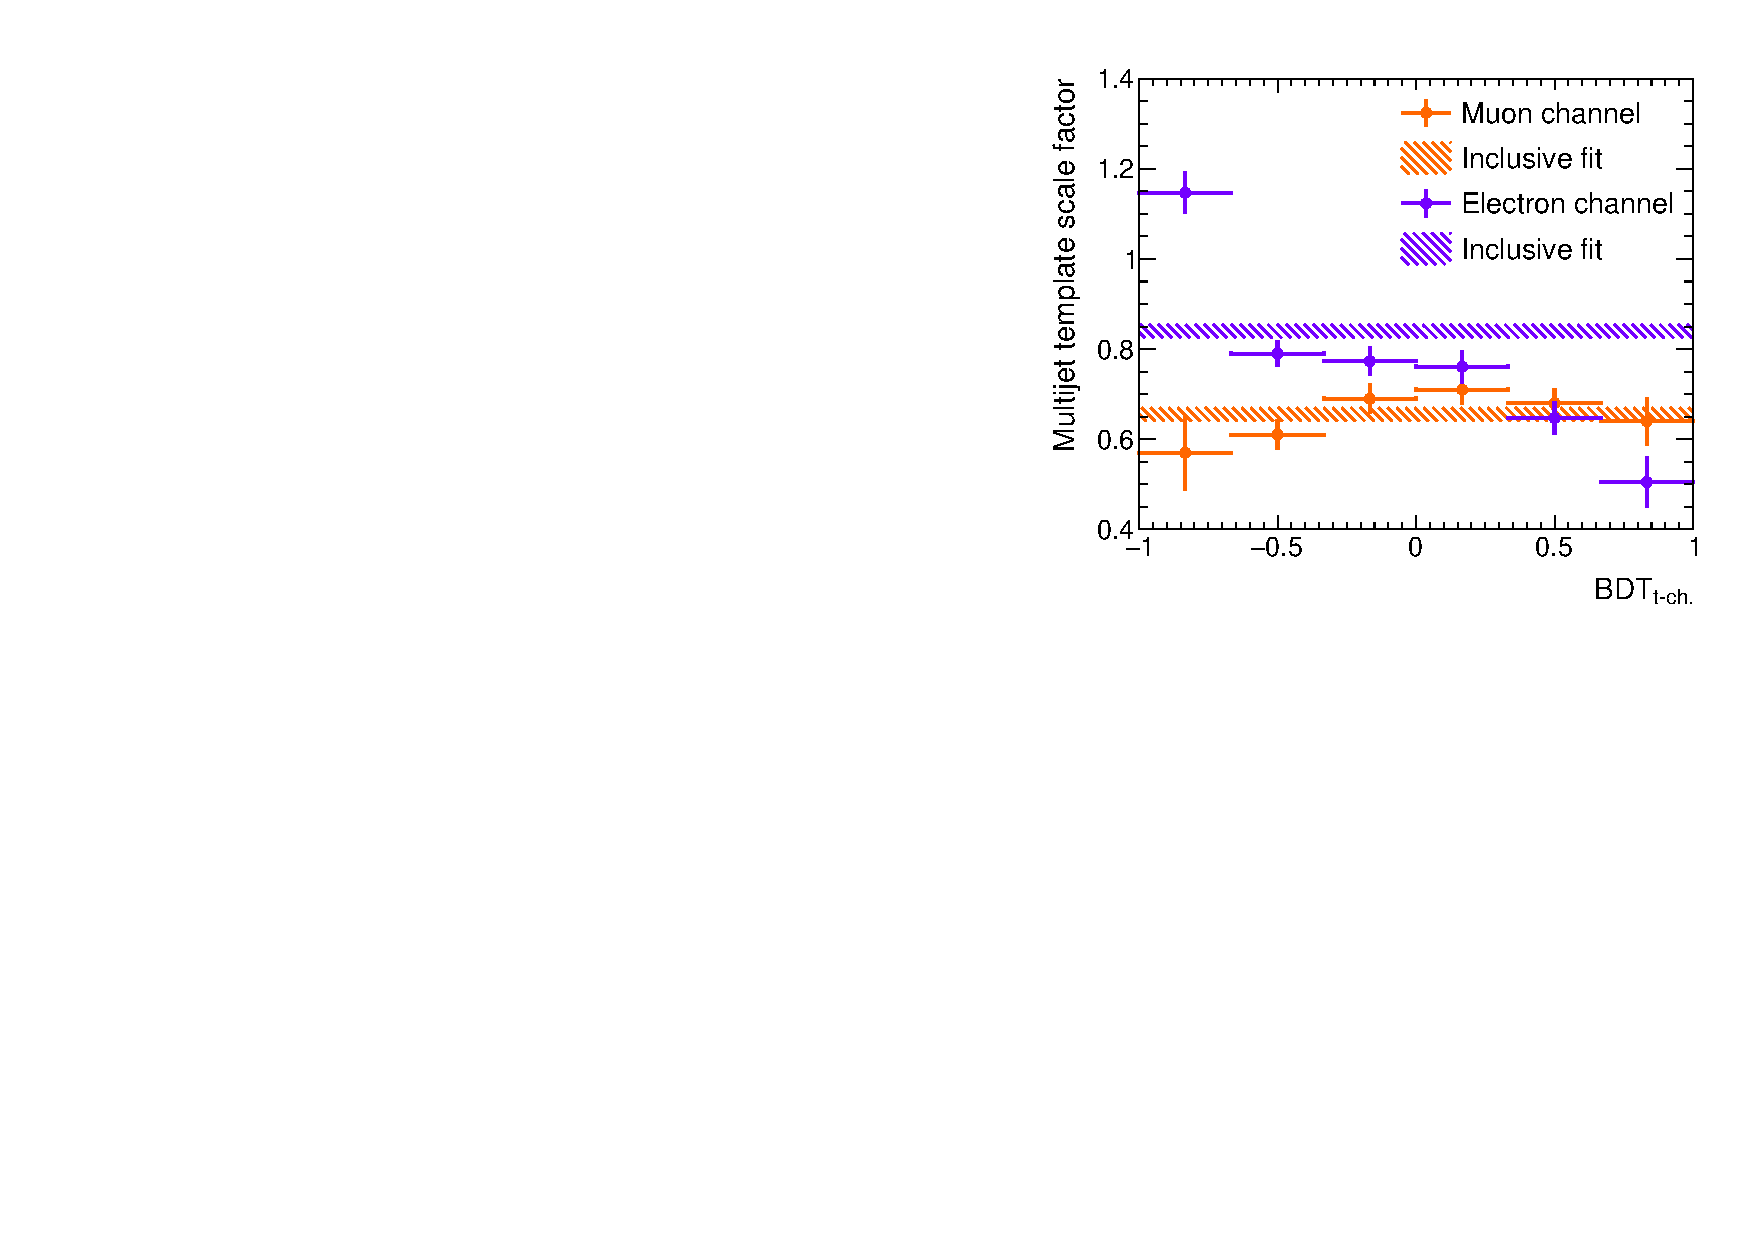
\includegraphics[width=0.55\textwidth]{figures/polarization/qcdStability.pdf}
}

Further investigations of the modeling of multijet events in the electron channel revealed that the distribution of the difference between the $\phi$ angles of the lepton and the missing transverse momentum is mismodeled. Figure~\ref{fig:polarization-dphi-lepton-met} shows the corresponding distributions in electron and muon channel. The $\Delta\phi$ distribution in the muon channel is instead well modeled by the multijet template.

\myfigure{\label{fig:polarization-dphi-lepton-met}Distributions of the angle in the transverse plane between the missing transverse momentum and the (a)~muon, (b)~electron after applying the described corrections.}{
\subfloat[]{\adjincludegraphics[height=4.8cm,trim={0 0 {0.16\width} 0},clip]{figures/polarization/afterBgCorr/2j0t/electron_2j0t_lepton_met_dphi_qcdnone_nol.pdf}}
\subfloat[]{\adjincludegraphics[height=4.8cm]{figures/polarization/afterBgCorr/2j0t/muon_2j0t_lepton_met_dphi_qcdnone.pdf}}
}

From these findings it is concluded that events from the sideband region provide an insufficient modeling of multijet events in the electron channel. The measurement of the top quark spin asymmetry is therefore only continued with data in the muon channel. This decision is further motivated by the result of a blind measurement on pseudo-data which showed that a combination of both channel will only result in an improvement of less than 5\% since the measurement is mainly limited by systematic uncertainties.

Further checks do not reveal any \todo{???} The analysis is unblinded in the muon channel. The distribution of the polarization angle in the muon channel is shown in Fig.~\ref{fig:polarization-cosTheta-SR-CR} in a signal-depleted and a signal-enriched region defined by $\bdttch<0$ and $\bdttch>0.45$ respectively. In the signal-depleted region, the distribution of data appears to be well modeled whereas in the signal-enhanced region a slight slope is observed.

\myfigure{\label{fig:polarization-cosTheta-SR-CR} Distributions of the polarization angle in (a)~signal-depleted and (b)~signal-enriched region in 2j1t muon channel.}{
\subfloat[]{\adjincludegraphics[height=4.8cm,trim={0 0 {0.16\width} 0},clip]{figures/polarization/afterBgCorr/2j1t/muon_2j1t_cosTheta_lj_CR_nol.pdf}}
\subfloat[]{\adjincludegraphics[height=4.8cm,trim={0 0 {0.16\width} 0},clip]{figures/polarization/afterBgCorr/2j1t/muon_2j1t_cosTheta_lj_SR_nol.pdf}}
}


%##############################################
\section{Unfolding}
%##############################################
\label{sec:polarization-unfolding}

After subtracting the remaining background contributions from data in the signal-enriched region, the reconstructed $\cos\theta_{\mu}^\star$ shape is unfolded to parton level and the spin asymmetry is extract from the differential cross section. The working point of the \bdttch discriminant which defines the signal-enriched region can be optimized such that .


is found by scanning the expected uncertainty of the measurement using pseudo-data as a function of the working point. The result is shown in Fig.~\ref{fig:polarization-bdtscan}. 

\myfigure{\label{fig:polarization-bdtscan}.}{
\adjincludegraphics[height=4.8cm]{figures/polarization/unfolding/scan_mu.pdf}
}



bdt cut, neyman construction, 2bin cross check, define angle for taus and not for tau decay products



\myfigure{\label{fig:polarization-neyman}.}{
\adjincludegraphics[height=4.8cm]{figures/polarization/unfolding/neyman_t_tbar.pdf}
}



%##############################################
\section{Statistical evaluation}
%##############################################

Q-scale reweighting, chi2 fit, symmetrizing  uncertainties

\mytable{}{
\begin{tabular}[htc]{|r | r  r  r |}
\hline 
 
        & $\delta \AmuT\cdot 10^{2}$
        & $\delta \AmuTbar\cdot 10^{2}$
        & $\delta \AmuTplusTbar\cdot 10^{2}$
         \\

\hline 
Statistical & $3.2$ \hspace{0.1cm}  & $4.6$ \hspace{0.1cm}  & $2.6$ \hspace{0.1cm}  \\
Limited MC & $2.1$ \hspace{0.1cm}  & $3.2$ \hspace{0.1cm}  & $1.8$ \hspace{0.1cm}  \\  
\gls{ml}-fit uncertainty & $0.7$ \hspace{0.1cm}  & $1.2$ \hspace{0.1cm}  & $0.6$ \hspace{0.1cm}  \\ 
Diboson fraction & $<0.1$ \hspace{0.1cm}  & $<0.1$ \hspace{0.1cm}  & $<0.1$ \hspace{0.1cm}  \\ 
\zjets fraction & $<0.1$ \hspace{0.1cm}  & $<0.1$ \hspace{0.1cm}  & $<0.1$ \hspace{0.1cm}  \\ 
$s$~channel fraction & $0.3$ \hspace{0.1cm}  & $0.2$ \hspace{0.1cm}  & $0.2$ \hspace{0.1cm}  \\ 
tW fraction & $0.1$ \hspace{0.1cm}  & $0.7$ \hspace{0.1cm}  & $0.2$ \hspace{0.1cm}  \\ 
Multijet shape & $0.5$ \hspace{0.1cm}  & $0.7$ \hspace{0.1cm}  & $0.5$ \hspace{0.1cm}  \\ 
Multijet yield & $1.9$ \hspace{0.1cm}  & $1.2$ \hspace{0.1cm}  & $1.7$ \hspace{0.1cm}  \\ 
\hline
b-tagging & $0.7$ \hspace{0.1cm}  & $1.2$ \hspace{0.1cm}  & $0.9$ \hspace{0.1cm}  \\ 
Mistagging & $<0.1$ \hspace{0.1cm}  & $0.1$ \hspace{0.1cm}  & $<0.1$ \hspace{0.1cm}  \\ 
\Acrlong{jer} & $2.7$ \hspace{0.1cm}  & $1.8$ \hspace{0.1cm}  & $2.0$ \hspace{0.1cm}  \\ 
\Acrlong{jec} & $1.3$ \hspace{0.1cm}  & $2.6$ \hspace{0.1cm}  & $1.1$ \hspace{0.1cm}  \\ 
Unclustered \met & $1.1$ \hspace{0.1cm}  & $3.3$ \hspace{0.1cm}  & $1.3$ \hspace{0.1cm}  \\ 
Pileup & $0.3$ \hspace{0.1cm}  & $0.2$ \hspace{0.1cm}  & $0.2$ \hspace{0.1cm}  \\ 
Muon identification & $<0.1$ \hspace{0.1cm}  & $<0.1$ \hspace{0.1cm}  & $<0.1$ \hspace{0.1cm}  \\ 
Muon isolation & $<0.1$ \hspace{0.1cm}  & $<0.1$ \hspace{0.1cm}  & $<0.1$ \hspace{0.1cm}  \\ 
Trigger efficiency & $<0.1$ \hspace{0.1cm}  & $<0.1$ \hspace{0.1cm}  & $<0.1$ \hspace{0.1cm}  \\ 
\hline
\ttbar top quark \pt reweighting & $0.3$ \hspace{0.1cm}  & $0.3$ \hspace{0.1cm}  & $0.3$ \hspace{0.1cm}  \\ 
\wjets W~boson \pt reweighting & $0.1$ \hspace{0.1cm}  & $0.1$ \hspace{0.1cm}  & $0.1$ \hspace{0.1cm}  \\ 
\wjets heavy flavor fraction & $4.7$ \hspace{0.1cm}  & $6.2$ \hspace{0.1cm}  & $5.3$ \hspace{0.1cm}  \\ 
\wjets light flavor fraction & $<0.1$ \hspace{0.1cm}  & $<0.1$ \hspace{0.1cm}  & $0.1$ \hspace{0.1cm}  \\ 
\wjets shape reweighting & $2.9$ \hspace{0.1cm}  & $3.4$ \hspace{0.1cm}  & $3.1$ \hspace{0.1cm}  \\ 
Unfolding bias & $2.5$ \hspace{0.1cm}  & $4.2$ \hspace{0.1cm}  & $3.1$ \hspace{0.1cm}  \\ 
\hline
Generator model & $1.6$ \hspace{0.1cm}  & $3.5$ \hspace{0.1cm}  & $0.3$ \hspace{0.1cm}  \\ 
Top quark mass & $1.9$ \hspace{0.1cm}  & $2.9$ \hspace{0.1cm}  & $1.8$ \hspace{0.1cm}  \\ 
$t$~channel fact./renorm. scale  & $0.2$ \hspace{0.1cm}  & $0.2$ \hspace{0.1cm}  & $0.2$ \hspace{0.1cm}  \\ 
\ttbar fact./renorm. scale & $2.2$ \hspace{0.1cm}  & $3.4$ \hspace{0.1cm}  & $2.7$ \hspace{0.1cm}  \\ 
\ttbar matching & $2.2$ \hspace{0.1cm}  & $0.5$ \hspace{0.1cm}  & $1.6$ \hspace{0.1cm}  \\ 
\wjets fact./renorm. scale & $3.7$ \hspace{0.1cm}  & $4.6$ \hspace{0.1cm}  & $4.0$ \hspace{0.1cm}  \\ 
\wjets matching & $3.8$ \hspace{0.1cm}  & $3.0$ \hspace{0.1cm}  & $3.4$ \hspace{0.1cm}  \\ 
\Acrlong{pdf} & $0.9$ \hspace{0.1cm}  & $1.6$ \hspace{0.1cm}  & $1.2$ \hspace{0.1cm}  \\ 
\hline 
Total uncertainty & $10.5$ \hspace{0.1cm}  & $13.8$ \hspace{0.1cm}  & $10.5$ \hspace{0.1cm}  \\ 
\hline 
\end{tabular}
}

%##############################################
\section{Results}
%##############################################

\myfigure{\label{fig:polarization-unfolded-costheta} The figures are taken from Ref.~\cite{Khachatryan:2015dzz}.}{
\subfloat[]{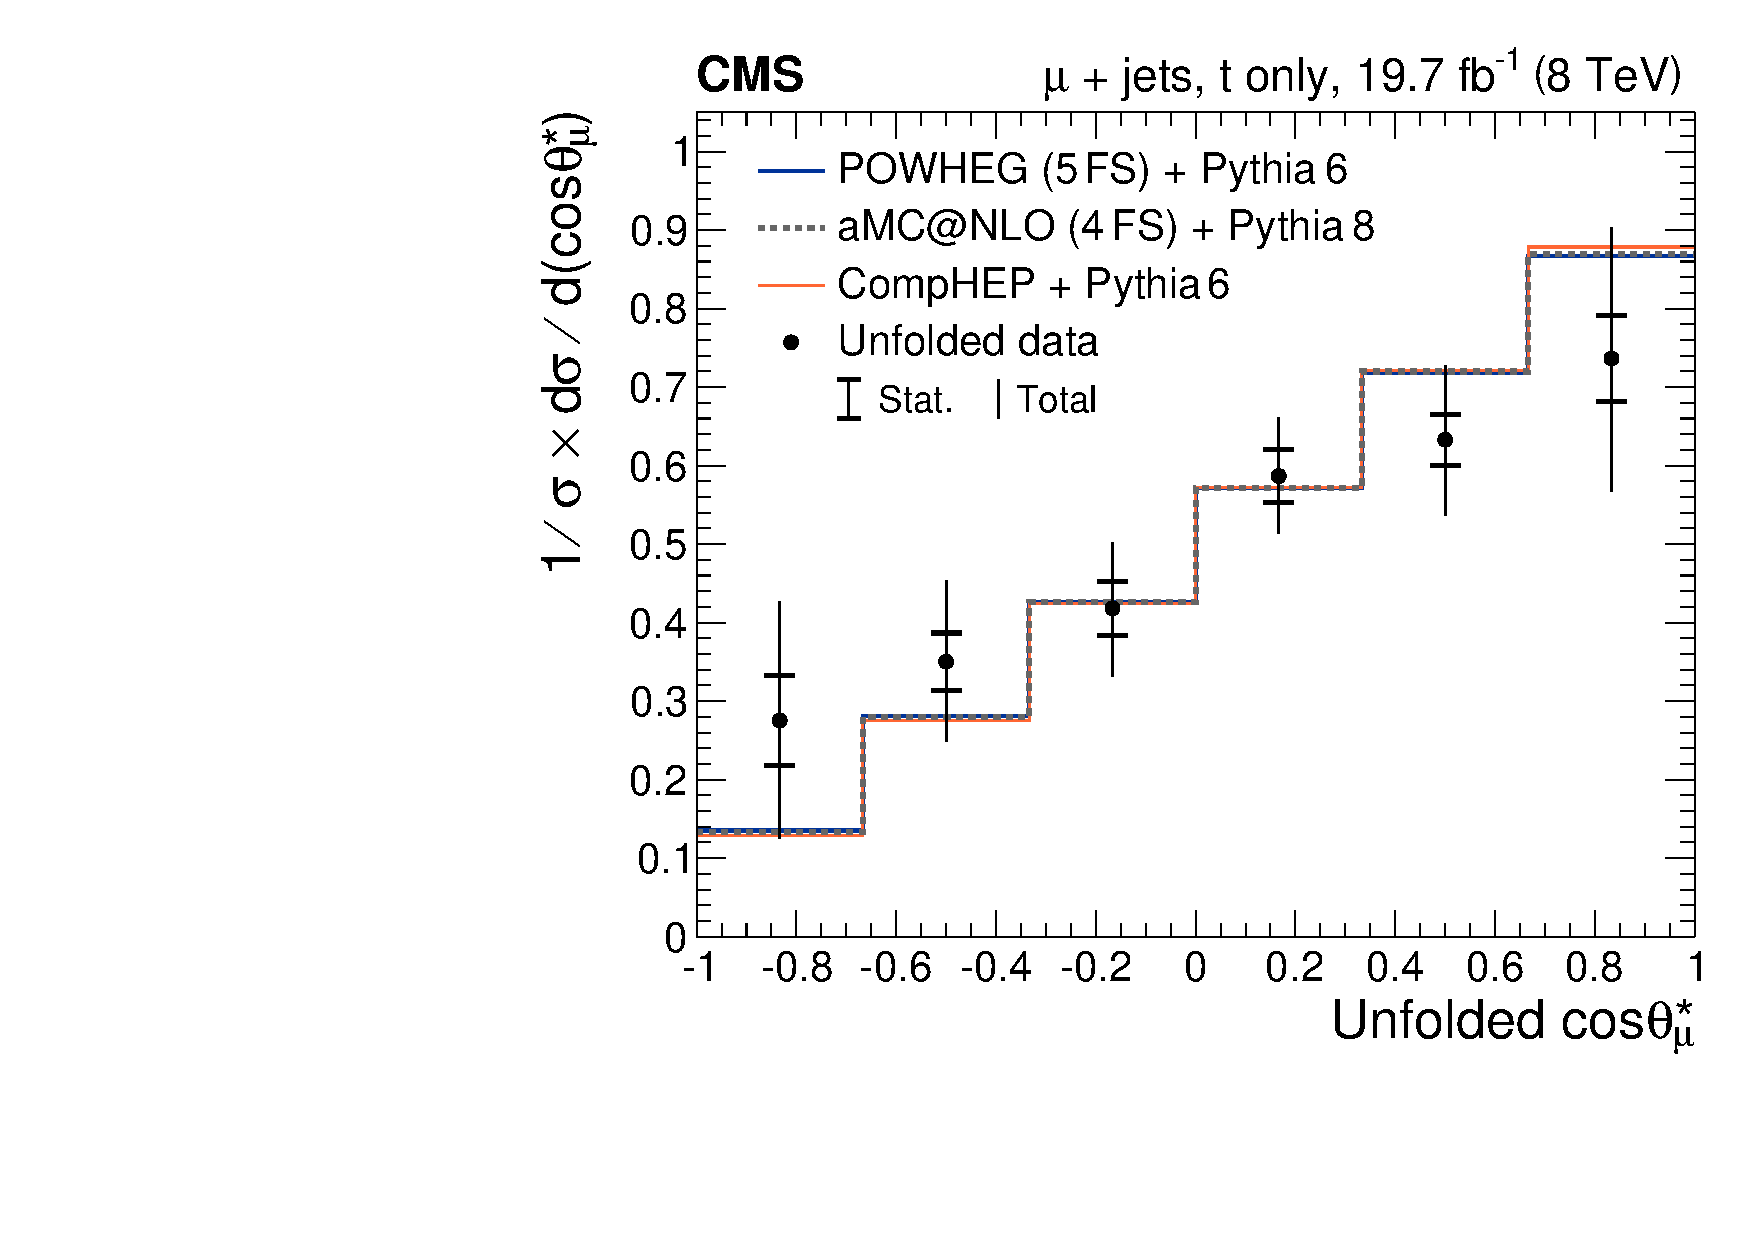
\includegraphics[width=0.48\textwidth]{figures/polarization/result/unfolded_mu_top.pdf}}
\hspace{0.02\textwidth}
\subfloat[]{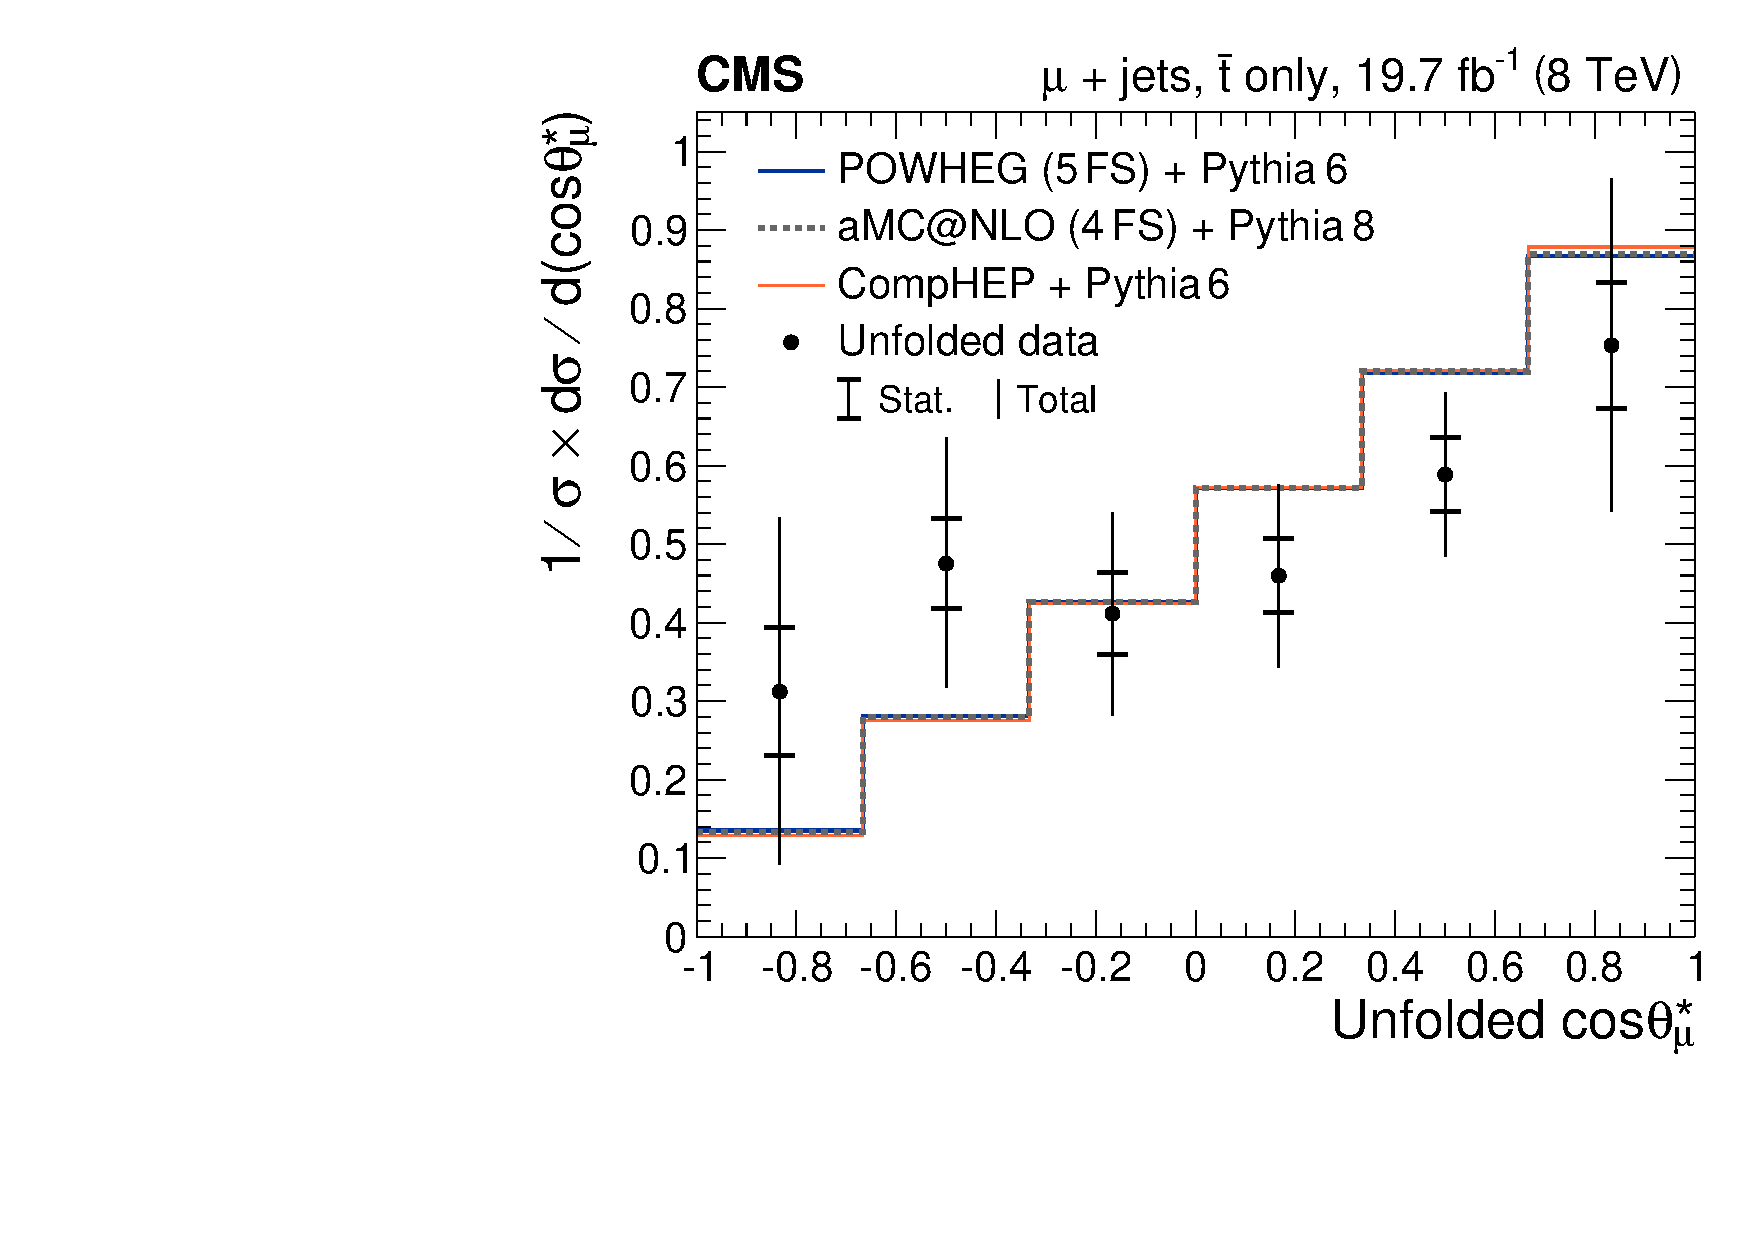
\includegraphics[width=0.48\textwidth]{figures/polarization/result/unfolded_mu_antitop.pdf}}\\
\subfloat[]{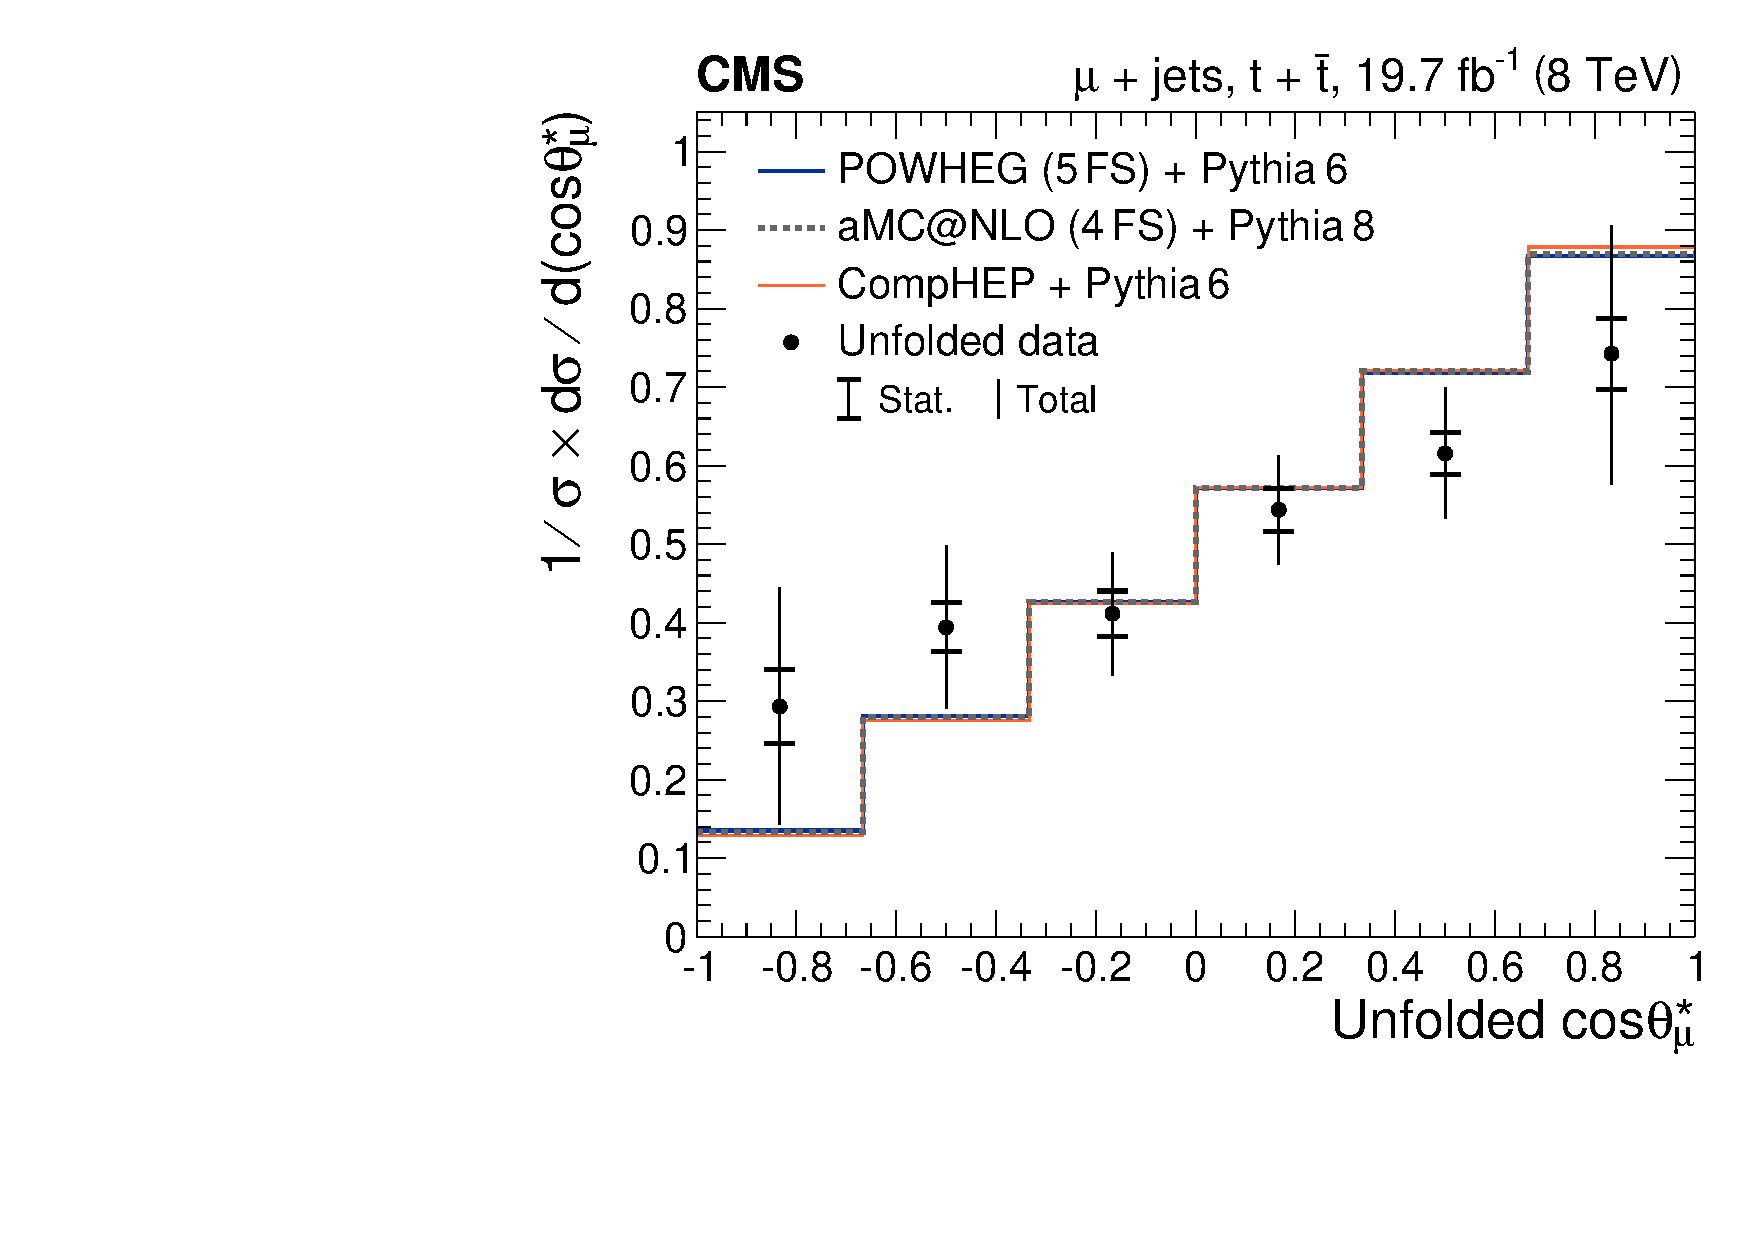
\includegraphics[width=0.48\textwidth]{figures/polarization/result/unfolded_mu.pdf}}
}


\myfigure{\label{fig:polarization-asymmetries}}{
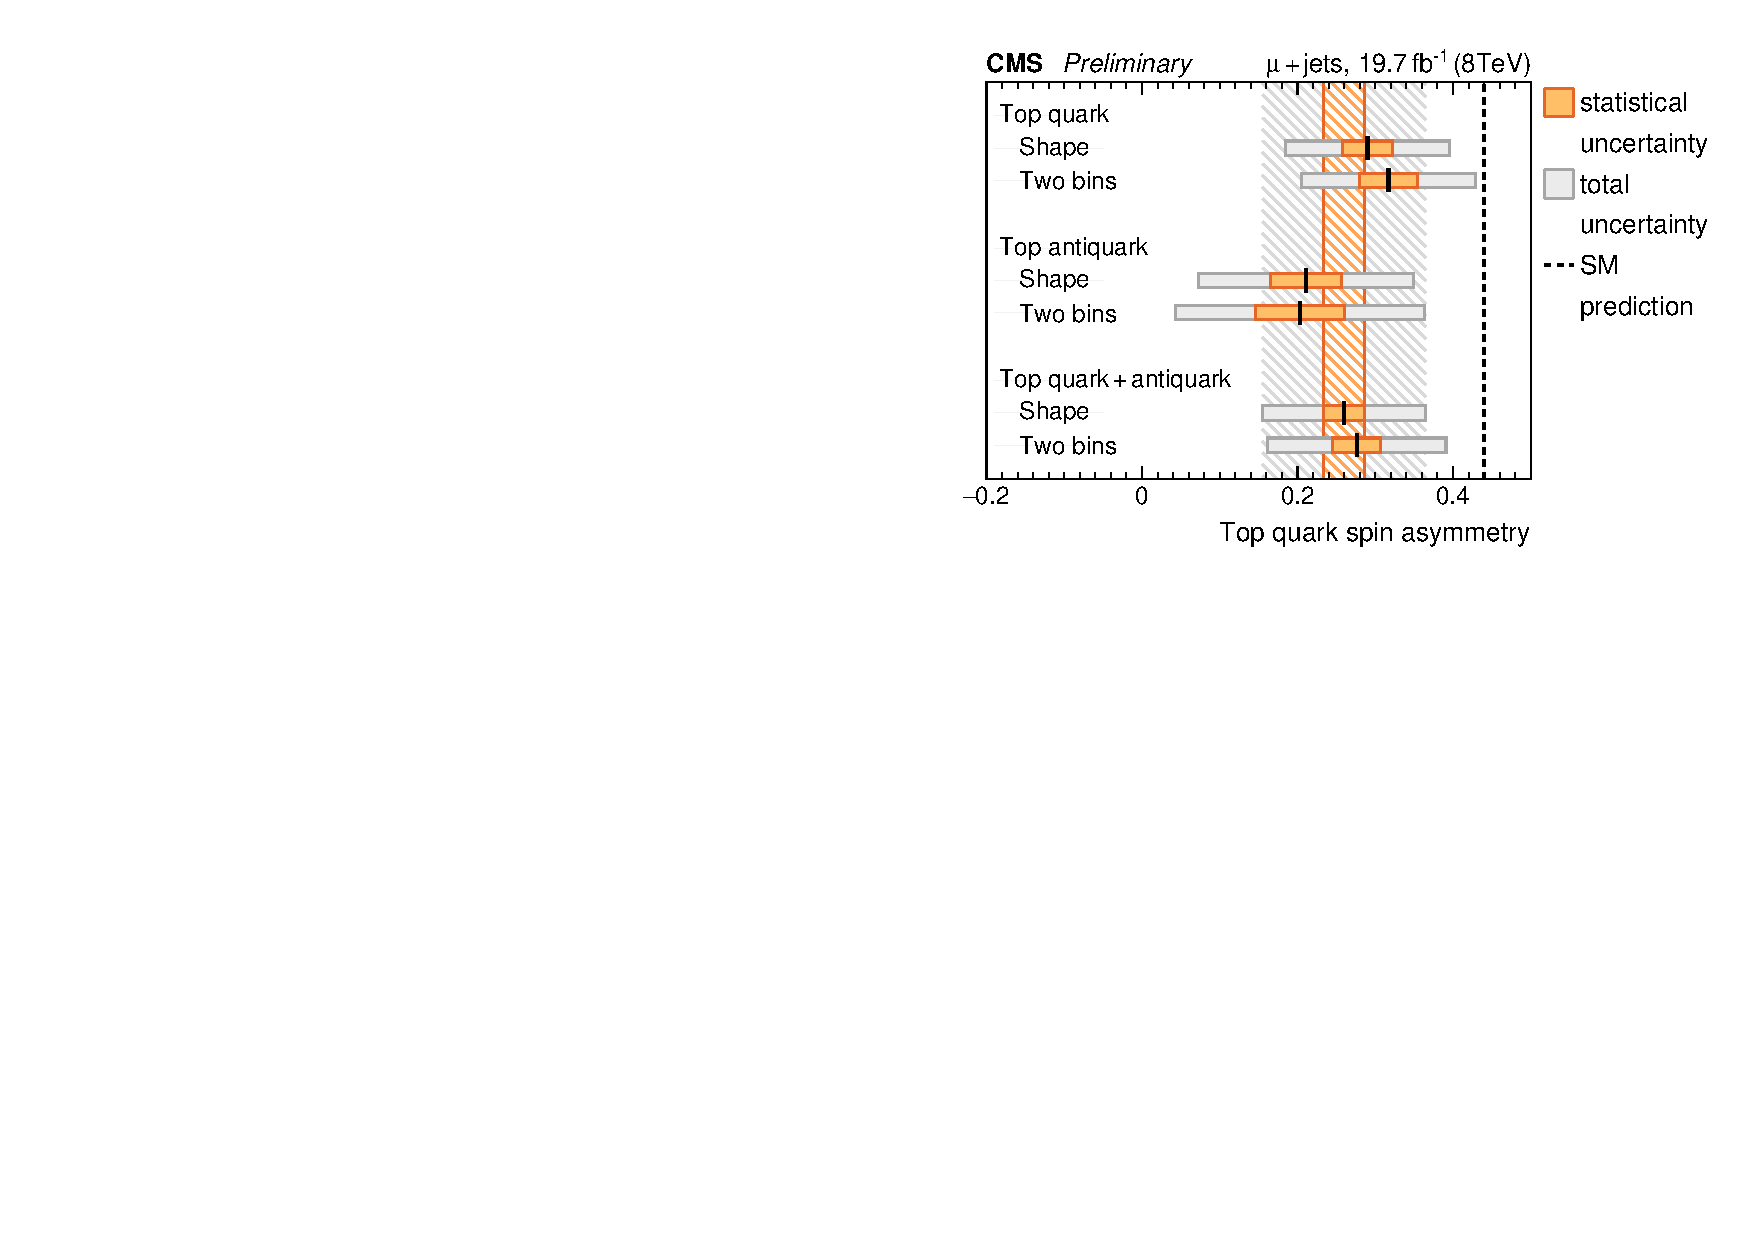
\includegraphics[width=0.7\textwidth]{figures/polarization/results.pdf}
}

\newcommand{\AlResultCombined}{\ensuremath{\Big[26.0\pm 10.5 \Big]\cdot 10^{-2}}\xspace}
\newcommand{\AlResultCombinedStatSys}{\ensuremath{\Big[26.0\pm 2.6 \mathrm{(stat.)}\pm 10.2\mathrm{(syst.)} \Big] \cdot 10^{-2}} \xspace}
\newcommand{\AlResultCombinedPvalue}{\ensuremath{4.6\cdot 10^{-2}}\xspace}

\newcommand{\AlResultTop}{\ensuremath{\Big[29.0\pm 10.5 \Big]\cdot 10^{-2}}\xspace}
\newcommand{\AlResultTopStatSys}{\ensuremath{\Big[29.0 \pm 3.2 \mathrm{(stat.)} \pm 10.0\mathrm{(syst.)} \Big]\cdot 10^{-2}}\xspace}
\newcommand{\AlResultTopPvalue}{\ensuremath{7.9\cdot 10^{-2}}\xspace}

\newcommand{\AlResultAntiTop}{\ensuremath{\Big[21.1\pm 13.8 \Big]\cdot 10^{-2}}\xspace}
\newcommand{\AlResultAntiTopStatSys}{\ensuremath{\Big[21.1\pm 4.6\mathrm{(stat.)}\pm 12.6\mathrm{(syst.)} \Big]\cdot 10^{-2}}\xspace}
\newcommand{\AlResultAntiTopPvalue}{\ensuremath{5.0\cdot 10^{-2}}\xspace}


From data, we measure

\begin{align}
\AmuT          & = \AlResultTopStatSys = \AlResultTop , \\
\AmuTbar       & = \AlResultAntiTopStatSys = \AlResultAntiTop , \\
\AmuTplusTbar & = \AlResultCombinedStatSys = \AlResultCombined
\end{align}

using TUnfold. The measured asymmetries are compatible with a p-value of

\begin{align}
\AmuT:&\hspace{0.3cm} p(\mathrm{data |SM})          = \AlResultTopPvalue , \\
\AmuTbar:&\hspace{0.3cm} p(\mathrm{data |SM})      = \AlResultAntiTopPvalue , \\
\AmuTplusTbar:&\hspace{0.3cm} p(\mathrm{data |SM}) = \AlResultCombinedPvalue
\end{align}

with the SM value of $43.8\cdot 10^{-2}$ as predicted by \POWHEG.



\begin{align}
\AmuT          & = \Big[31.7\pm 3.7 \mathrm{(stat.)}\pm 10.9\mathrm{(syst.)} \Big]\cdot 10^{-2} = \Big[31.7\pm 11.2 \Big]\cdot 10^{-2} , \\
\AmuTbar       & = \Big[20.3\pm 5.7 \mathrm{(stat.)}\pm 15.0\mathrm{(syst.)} \Big]\cdot 10^{-2} = \Big[20.3\pm 16.0 \Big]\cdot 10^{-2} , \\
\AmuTplusTbar & = \Big[27.6\pm 3.1 \mathrm{(stat.)}\pm 11.1\mathrm{(syst.)} \Big]\cdot 10^{-2} = \Big[27.6\pm 11.5 \Big]\cdot 10^{-2} 
\end{align}

using the 2-bin analytic unfolding method as cross check.



%##############################################
\section{Limits on anomalous couplings}
%##############################################

topfit

combine: t-channel 8TeV~\cite{Khachatryan:2014iya}, Whelicity at 8TeV~\cite{Khachatryan:2016fky}


\myfigure{\label{fig:polarization-limits}Projections of limits on anomalous couplings and the top quark polarization for cases with free floating polarization~(violet) or when fixing the polarization to the anomalous couplings~(orange): (a)~left-handed vector couplings against polarization; (b)~right-handed vector coupling against polarization; (c)~left-handed tensor coupling against polarization; (d)~right-handed tensor coupling against polarization.}{
\subfloat[]{\adjincludegraphics[height=4.65cm,trim={0 0 {0.15\width} 0},clip]{figures/polarization/limits/Ptvl-nol.pdf}}
\subfloat[]{\adjincludegraphics[height=4.65cm,trim={0 0 {0.0\width} 0},clip]{figures/polarization/limits/Ptvr.pdf}}\\
\subfloat[]{\adjincludegraphics[height=4.65cm,trim={0 0 {0.15\width} 0},clip]{figures/polarization/limits/Ptgl-nol.pdf}}
\subfloat[]{\adjincludegraphics[height=4.65cm,trim={0 0 {0.0\width} 0},clip]{figures/polarization/limits/Ptgr.pdf}}
}
